\documentclass[12pt]{article}
\usepackage[margin=.25in]{geometry}
\usepackage{textcomp}
\usepackage{float, graphicx, color, soul}
\usepackage{amsmath}
\usepackage{listings}
\lstset{
basicstyle=\ttfamily,
frame=single,
numbers=left
}
\title{CS185C: \\ 
Final Project \\
Malware Classification}

\author{Jordan Conragan,  Brett Dispoto}

\begin{document}
\maketitle
\tableofcontents
\newpage

\part{Abstract and Introduction}
  Intro
\hl{Add table for best model}

\part{Methodology and Dataset}
%Talk about the dataset, 
%Features,
%imbalanced classes,
%which families we use
%preprocessing
\section{Preprocessing the Dataset}
\hl{Specify which families were used}
Most of the machine learning techniques used in this report use variants of the same preprocessing steps. Here are the preprocessing steps taken for the methods described in this report. Preprocessing was done using both python and bash scripts. The relevant files can be found in the \texttt{preprocessingScipts} directory of our submission.
  \begin{enumerate}
  \item Download the dataset (\texttt{malicia} | provided by Fabio Di'Troia).
    \item Split the dataset into directories based upon their family label. (Already completed by the dataset provider.)
    \item For each malware family, the following steps were then taken:
      \begin{enumerate}
        \item Read through all of the files, count the occurrence of each unique opcode across all files.
        \item Take the $n$ (turning parameter) most common Opcodes, and convert them to an ASCII symbol for observation symbols for our HMMs. The Opcodes which are not within the $n$ most common will be converted to an "other" symbol. This will reduce noise in our model.
        \item Once each opcode is assigned a symbol, we again read through the files and convert the opcodes to symbols.

        \begin{enumerate}
          \item If bagging is being used, make copies of \textbf{each} converted malware file, which will later be split up accordingly during training.
          \item Otherwise, if boosting or stacking is being used, we can simply dump the converted opcodes (symbols) for the entire family into one huge file. This file will be our observation sequence.
        \end{enumerate}
      \end{enumerate}
  \end{enumerate}




\part{Experimental Setup}
\section{K-Nearest Neighbors}
K-Nearest Neighbors (KNN) was one of the first algorithms implemented in this work. KNN makes a wise first choise because it allows us to examine the dataset, potentially for intuitive solutions to building a model.

KNN was implemented following according to the following features of our samples:
  \begin{enumerate}
    \item Entropy of opcode sequence, and
    \item Number of distinct opcodes
  \end{enumerate}
  KNN is performed using the files \texttt{KNN.py} and \texttt{knnPreprocesor.py}. The procedures and results are described in the sections below. \textit{sklearn} was used as a KNN library for python.

\subsection{KNN Procedure}
  Procedures for running the KNN algorithm on the dataset is as follows:
  \begin{enumerate}
    \item Preprocess the dataset. This includes:
        \begin{enumerate}
          \item Convert all opcodes to symbols,
          \item Count the number of distinct symbols in each sample,
          \item Compute the entropy $H(X)$ of the sequence of opcodes. This is given by Shannon's Entropy:
          \begin{equation}
            H(x) = E[I_X] 
          \end{equation}
        \item Write the above information in a file for each sample.
        \end{enumerate}
      \item Use 90\% of the dataset as our "training" samples (there really is no training in KNN).
      \item Test KNN using 10\% of the dataset.
      \item Repeat steps 2 and 3 for different values of $K$, ranging from $2$ to $10$. Keep the best result.
  \end{enumerate}

\section{HMM Boosting}
  \subsection{HMM Boosting Procedure}
  Boosting was done according to the procedure described in lecture. That is, all HMMs of a malware family were trained using the same observation, only with different training parameters (random seeds) varying across models. \textit{HiddenMarkovModel.java} and \textit{Boosting.java} are the files where boosting is implemented.
 
\section{Stacking}
  \subsection{Stacking Procedure}
  Beause stacking yielded the best results among all tested models, most extensive hyperparameter tuning was performed using stacking. Stacking is implemented using the files \textit{Stacking.java}, \textit{Stacking.python}, \textit{HiddenMarkovModel.java}, in addition to the library LibSVM. Stacking is implemented using HMMs as weak classifiers, then using SVMs as metaclassifiers, using "one-vs-everything else"  methodology to achive multiclass classification using support vector machines.

The procedure for each component of the classifier:
\paragraph{HMM Training}
\begin{lstlisting}
HMMs for winwebsec was trained on 1000 files
HMMs for zbot were trained on 1067 files
HMMs for zeroaccess were trained on 651 files
\end{lstlisting}


\paragraph{SVM Training}
\begin{lstlisting}
SVM for winwebsec was trained on the scores from 5 
  HMMs of 1089 winwebsec files and 1720 total files from zbot and zeroaccess
SVM for zbot was trained on the scores from 5 HMMs
  of 533 zbot files and 2832 total files from winwebsec and zeroaccess
SVM for zeroaccess was trained on the scores from 5 HMMs of 325 zeroaccess 
  files and 3206 total files from winwebsec and zbot
\end{lstlisting}

\paragraph{Testing SVM}
\begin{lstlisting}
SVM for winwebsec was tested on the scores from 5 HMMs of 1089 winwebsec
  files and 1719 total files from zbot and zeroaccess
SVM for zbot was tested on the scores from 5 HMMs of 533 zbot files and 
  2831 total files from winwebsec and zeroaccess
SVM for zeroaccess was tested on the scores from 5 HMMs of 326 zeroaccess 
  files and 3247 total files from winwebsec and zbot
\end{lstlisting}



\section{HMM Bagging}
  Bagging is performed using the files \texttt{Bagging.java} and \texttt{HiddenMarkovModel.java}. The procedures and results are described in the sections below.
\subsection{Bagging Procedure}
  The following steps were performed in order to use bagging as an ensemble method:
  \begin{enumerate}
    \item Split assembly instructions into their appropriate family, and translate the instructions to HMM symbols,
    \item Within these family folders, use a shell script (included, \texttt{makeTesting.sh}) in order to split 10 percent of the samples into a test set.
    \item Train $x$ HMMs on each family,
    \item Once each HMM for a given family is trained, score the observation sequence which just used to train the model.
    \item Write down this score. 
    \item Once all HMMs of a given family are trained, use whichever ensembler aggregate function to take all the generated scores and aggregate them into one score. 
    \item Once training is complete for all families, for each family we now have this "aggregate score" written down in a log in the directory where the training samples are located.
    \item Finally, to test all of these trained HMMs, we go into all of the test sets, score the test sample using the \textbf{each of the three "ensemblers"} (each made up of $x$ HMMs.). Once we have the score from each ensembler, we can then go back to the logs where the original score was written down for the training samples. 
    \item Now, our sample has one score for each ensembler, denoted as $S_{1..\text{\texttt{num\_ensembler}}}(x_{\text{test}})$
    \item We classify this sample as whichever has the minimum of $abs(S_{\text{\textit{family}}}(x_{\text{test}}) - \text{\textit{score}}_\text{family} )$, that is, we classify as whichever family's "original score" score is closest to the score for the sample given by \textit{that family's} "ensembled" HMMs. In other words, we're just doing the KNN algorithm, where $k = 1$
  \end{enumerate}


\newpage
\part{Experimental Results}
\hl{Specify hyperparam N, M, etc..... for every model}


  \subsection{KNN Results}
  Below are the results of the above procedure:

          \begin{figure}[H]
          \centering
          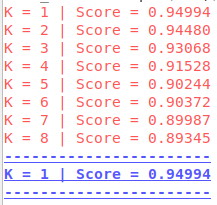
\includegraphics[width=0.3\textwidth]{knn.png}
          \caption{Finding the best value for $k$.}
          \end{figure}
 
  As can be seen above, the best achived accuracy using KNN is where $K=1$.
  
          \begin{figure}[H]
          \centering
          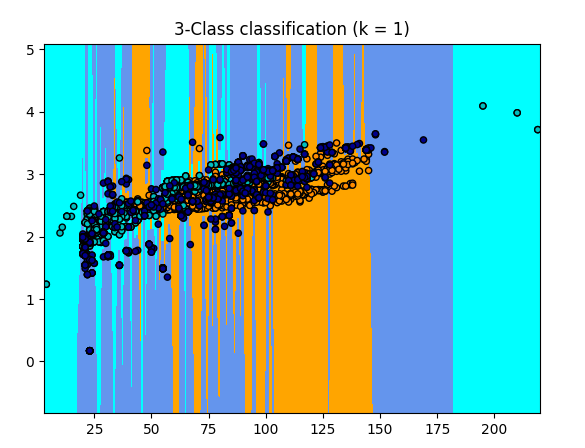
\includegraphics[width=0.55\textwidth]{k1.png}
          \caption{Family clusters when $K=1$}
          \end{figure}
 
  When we plot the clusters on a graph, we can see that when $K = 1$, we can see that we're overfitting on the training set:


  Therefore, if this model were used in software production, we would probably choose a larger $K$ such as $K=3$ as to reduce overfitting, despite the fact that $K=3$ yields lower accuracy. Below are the clusters when $K=3$:
          \begin{figure}[H]
          \centering
          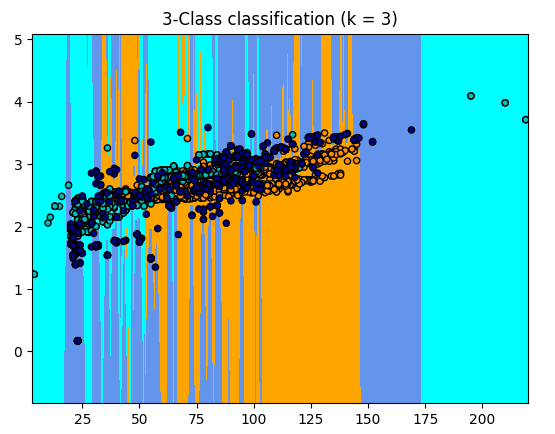
\includegraphics[width=0.5\textwidth]{k3.png}
          \caption{Family clusters when $K=3$}
          \end{figure}
  \subsubsection{KNN N-Fold Validation}
  \hl{Not yet implemented}

 \subsection{Boosting Results}
Whether the score of the file was determined by the average or by the maximum value of the scores of 5 randomly restarted HMMs, the Boosting experiments did not yield a useful classifier. This can be clearly seen by the ROC curve (which was created where N = 2, the number of unique opcodes = 35, and the scores from the HMMs were averaged) where the true positive rate and false positive rate are all over the place. A more intuitive way of understanding why this method failed is to compare the scores of 5 randomly chosen files from the same family the HMMs were trained on and the scores from 5 files of a different family than the HMMs were trained on. 
for example:
\begin{lstlisting}
5 random score from family X
Score 1: -17102.39110157962
Score 2: -2453.0432816283646
Score 3: -24443.862815912897
Score 4: -771.3044309566772
Score 5: -2648.110295014743
\end{lstlisting}
\begin{lstlisting}
5 random scores from family Y
Score 1: -22302.30088705916
Score 2: 8179.418459861058
Score 3: 10555.795790797403
Score 4: 7972.734255134028
Score 5: 9193.531925297084
\end{lstlisting}
It is easy to see that a simple threshold is not sufficient to categorize a file as either malware from the same family the HMMs were trained on or malware from a different family. Different hyperparameters were tested, such as letting N = 3, 4, 5, or letting the number of unique opcodes be 20, 30, and 40. Each one yielded a similar result. It is possible that the HMMs are overfitting, and so performing some sort of cross validation would produce better results, but due to the overwhelming success of the Stacking experiments (next section), this was not pursued.
\begin{figure}[H]
\centering
\includegraphics[width=0.45\textwidth]{Boosting.png}
\caption{ROC Curve where $N=2$.}
\end{figure}

  \subsection{Stacking Results}
  \begin{table}[H]
    \centering
  \begin{tabular}{|l|l|l|}
    \hline \textbf{Key} & \textbf{Value} \\\hline \hline
  N                   &        $ 5                    $\\\hline
  Unique Opcodes      &        $ 35                   $\\\hline       
  Max Iterations      &        $ 100                  $\\\hline 
  SVM Parameters      &        $ c = 2, g = 2^{-16}   $\\\hline 
  \hl{WinWebSec Accuracy } &   $ 98.9324\% (2780/2810)$\\\hline 
  \hl{Zbot Accuracy      } &   $ 98.366\% (3311/3366) $\\\hline 
  \hl{ZeroAccess Accuracy} &   $ 98.4615\% (3520/3575)$\\\hline 
  \end{tabular}
  \end{table}  

  \begin{figure}[H]
  \centering
  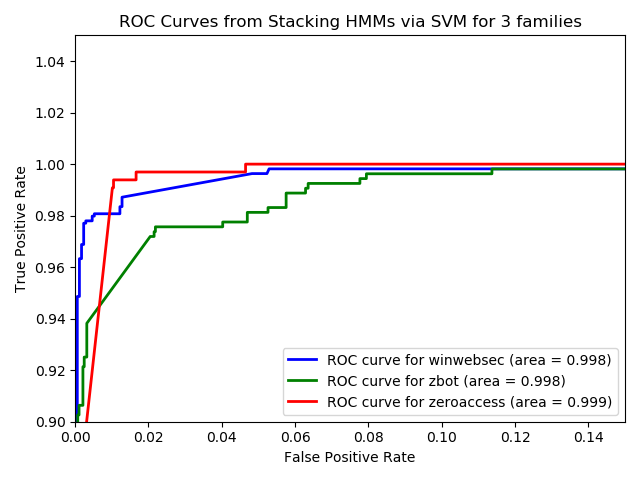
\includegraphics[width=0.66\textwidth]{stacking.png}
  \caption{ROC Curve where $N=2$.}
  \end{figure}
\paragraph{Logistics}
  Each family was split by 50\%, 25\%, and 25\%. 50\% of the family trains the HMMs. 25\% trains the SVM, and the final 25\% tests the SVM. It took well over an hour and a half to train all 15 HMMs used for these experiments, and though multithreading was implemented, our workstation was running out of memory when training with large observation sequences.
\paragraph{Hyperparameter Tuning}
  \subparagraph{Number of Opcodes}
  The number of unique opcodes for the best found classifier was 35. Originally tests were perfromed with 32 unique opcodes and got good results from that. Then 30 and 40 unique opcodes were tried, getting slightly worse results. Finally 35 opcodes was tested, which yielded slightly better results. The difference between 32 and 35 opcodes could just have been due to a lucky random restart, but it does seem like 35 opcodes is reliably better than 30 and 40 (the exact scores I got have unfortunately been lost). Finally, I tried 20 opcodes, getting significantly worse results.
  \subparagraph{Number of HMMs}
  Stacking was tried with scores from 3, 5 and 6 different HMMs. 5 and 6 HMMs were comparable in accuracy and differences were likely caused by the random restarts. However, since it took 20\% longer to train 6 HMMs, not many experiments were performed with them, so it is possible that there was some further way to optimize them beyond what I could do with 5 HMMs.
  \subparagraph{HMM Tuning}
 For the HMMs themselves, N = 2, 3, 4, and 5 were tried. N = 4 and 5 were comparable in accuracy, though N= 5 seems to have been slightly better (once again, possibly just due to randomness). N = 2 and 3 were outclassed by 4 and 5 by at least 2-3\%. N = 5 takes longer to train and uses more memory, but there is a reason I chose it over N = 4, and it has to due with the hyperparameters for the SVM described below.
  \subparagraph{SVM Tuning}
  Finally, we get to the SVM. The library used was Libsvm version 3.24. There are a couple of SVMs that Libsvm supports, so we chose the default \textsc{c-svc}. For the SVM kernel, the Radial Basis Function (RBF) kernel was used, which also happens to be the default kernel. Libsvm offers other kernels, such as a linear, polynomial, and sigmoid kernel. The linear kernel yielded horrible results (54\% - 60\%, little better than guessing) and every other available kernel would cause an \textit{MAX\_ITERATIONS\_REACHED} error from LibSVM.
  \subparagraph{Library Specific Tuning}
  Per the suggestion of the creators of Libsvm, there are two hyperparameters, $c$ (budget) and gamma (RBF kernel parameter), that I should tweak. If appropate values are chosen for these hyperparmeters,the testing accuracy can be drastically increased, but if the wrong values are chosen, then accuracies tend to then range from 60-80\%, which is obviously suboptimal.  We found through experimentation (choosing values c = $2^2$ through $2^-15$) that letting c = 2 is pretty much optimal for every family, for any number of HMMs with any N, and for any gamma value for the SVM. It is possible that we could have optimized these hyperparameters more by searching through smaller itervals such as $c = 1.9, 1.8, 1.7, ... 2.1, 2.2, .....$ but at that point, we would basically just be optimizing the SVM for the test set of the family, and while that would definitely be good to eek out the highest score in a competition, it probably wouldn't make the model better overall. Finally, we get to gamma. Choosing a good value for gamma is just as important as choosing a good value for c. We found experimentally that good values range between $2^{-10}$ and $2^{-20}$, although choosing the right one between those limits could mean a difference in accuracy of 5\% or more.
The proper gamma value seemed to change with N, the number of files that are being used in the training set for the HMM/SVM, and random chance from the randomly restarted HMMs. When N = 4, it was difficult to find a single gamma value that would give a consistent result for all 3 families at once. Each family would be 1-5\% less accurate than the last (although this did allow me to reach a 99.3007\% accuracy on ZeroAccess). However, when N = 5, I found that I could find a gamma value where all families would be about equally accurate (in the 98.5\% range). 

\subsection{Bagging Results}
  The best found bagging results are given in the below table:
  \begin{table}[H]
    \centering
  \begin{tabular}{|l|l|l|}
    \hline \textbf{Key} & \textbf{Value} \\\hline \hline
    Ensembler Aggregate Function & \textsc{MAX}  \\ \hline
    HMM's per ensembler & 10 \\ \hline
    N (HMM parameter -- \# states) & 2 \\ \hline
    Random initialization seed (HMM) & 0 \\ \hline
    Test set size  & 10\% of training set \\ \hline
  \hl{Test Accuracy} & \hl{0.9974326059050064}  \\ \hline
  \end{tabular}
  \end{table}  
  As is shown in the table above, the first bagging experiments went well on the surface. 

  \paragraph{On the Result:}
  \begin{enumerate}
    \item Whenever a sample was scored \textbf{using an HMM which was NOT trained on the family which the sample belongs to, the score is returned as NaN.} This makes for very good accuracy; however, this behaver cannot be mathematically or otherwise justified.
      \begin{itemize}
        \item For example, if a \texttt{winwebsec} sample was scored using an HMM which was trained on samples form the \texttt{zbot} family, then all the \texttt{zbot} HMMs will give \texttt{winwebsec} samples a score of NaN. \textit{This was somewhat unexpected, because our HidddenMarkovModel implementation takes special caution (using logrythims) to avoid underflow. Further, we know our HMM is valid because of extensive testing using Mark Stamp's paper "A Revealing Introduction to Hidden Markov Models"}. Our intuition tells us that this is okay, because the samples are still being given a valid score when the correct family's HMM's is used.
        \item To attempt to remedy this, we tried changing training methodology:
          \begin{enumerate}
            \item \textbf{Increase number of HMMs} | Currently, durring training, when an HMM is trained on an observation sequence, that observation sequence is much, much larger than the actual samples which are being scored. To remedy this, we can split our "ensemblers" into more "bags" such that they're made up of more HMMs. In turn, each HMM will be trained on a closer amount of data it will be tested on. Despite our rationale.... results from splitting the ensemblers into 30 or 100 HMMs each rather than 10 yielded the \textit{exact same results.}.
        \item Originally, the plan was to add an SVM on top of the bagging described here. However, because samples of the "wrong" family are always given a score of \texttt{NaN}, this would be completely useless.
          \end{enumerate}
     \end{itemize}
  \end{enumerate}



\end{document}

\iffalse
Todo:
  Sample with replacement for training baggging HMM.

  SVM using the same features as the KNN tests

  Add N-Fold to KNN

  DONE Do some ML method (perhaps KNN) where features could be:
  -Entropy
  -Number of distinct opcodes

  Add N-fold validation to bagging
  Trying bagging with replacement
  Use ROC curves

  Add random forrest somewhere?
\fi
